\documentclass[a4paper,12pt]{report}

\usepackage{alltt, fancyvrb, url}
\usepackage{amssymb}
\usepackage{cleveref}
\usepackage{graphicx}
\usepackage{subfigure}
\usepackage{wrapfig}
\usepackage{amsmath,amssymb,stmaryrd,mathtools,alltt}
\usepackage{algorithmic, algorithm}
\usepackage[utf8]{inputenc}
\usepackage{fontenc}
\usepackage{url}
\usepackage{cleveref,amsmath,amssymb,stmaryrd,mathtools,alltt,algorithm}
\usepackage{amssymb}

% Questo commentalo se vuoi scrivere in inglese.
\usepackage[italian]{babel}

\title{Damiano gay}
 
\author{Danilo Pianini}
\date{\today}


\begin{document}
 
% Prima pagina gratis
\maketitle

% menu gratis
\tableofcontents
 
\chapter{Capitolo}
\section{Sezione}
\subsection{Sotto Sezione}
\subsubsection{Sotto sotto Sezione}
\begin{itemize}
 \item Questo
 \item elenco
 \item non
 \item è
 \item numerato
\end{itemize}
\begin{enumerate}
 \item Questo
 \item elenco
 \item è
 \item numerato
\end{enumerate}

Si può scrivere in \textbf{grassetto}, \textsc{maiuscoletto}, in \textit{corsivo}, \emph{enfatizzato} (ovvero sceglie \LaTeX in base al testo che lo circonda), \underline{sottolineato}, \texttt{equispaziato} (ottimo per il codice, ad esempio \texttt{public static void main(String[] a)})

\begin{verbatim}
clear
clc
TA=EMGDATA1(1,:);
GC_filtrato=filtfilt(num,den,GC_abs);
figure(3);
plot(TA_filtrato)
figure(4);
plot(GC_filtrato)
for i=1:151
    EMG_GC_filtrato(1,i)=mean(GC_filtrato(:,(100*(i-1)+1):(100*i)));
end
\end{verbatim}

\tiny
tiny

\scriptsize
scriptsize

\footnotesize
footnotesize

\small
small

\normalsize
normalsize (default)

\large
large

\Large
Large (capital "L")

\LARGE
LARGE (all caps)

\huge
huge

\Huge
Huge (capital "H")

\normalsize
\begin{equation}
a_i^n
\end{equation}

\begin{figure}
  \begin{center}
    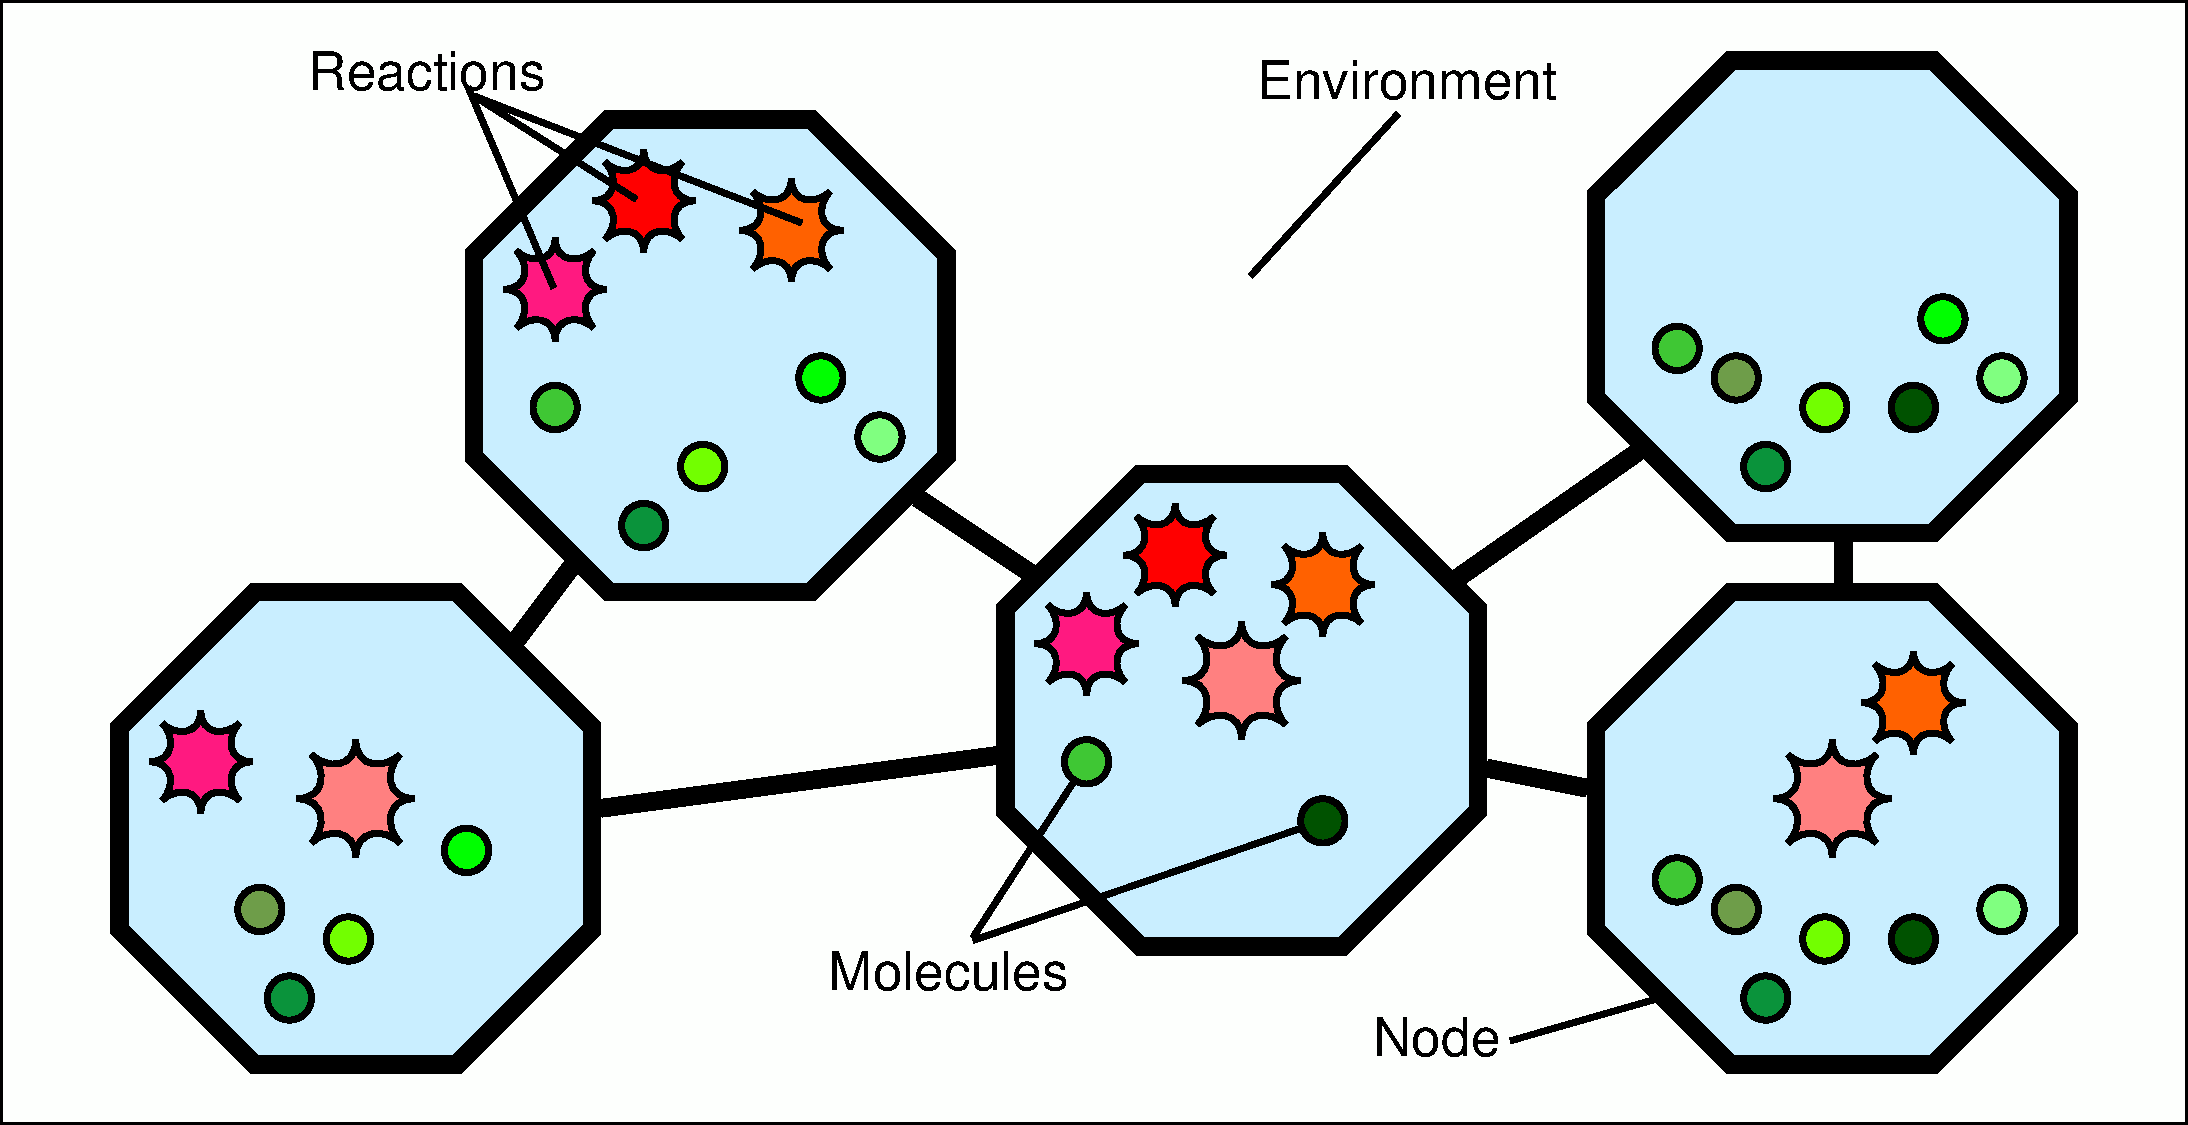
\includegraphics[width=0.99\columnwidth]{images/model.pdf}
    \caption{computational model: it features a possibly continuous space embedding a linking rule and containing nodes. Each node is programmed with a set of reactions and contains a set of structured molecules.}
    \label{img:model}
  \end{center}
\end{figure}

Puoi usare le label per fare i riferimenti, tipo l'Immagine \ref{img:model}. Per le citazioni, si usa \cite{papero}.



% scegli lo stile, e la bibliografia è gratis
\bibliographystyle{abbrv}
% questo file deve contenere i bibtex.
\bibliography{template}

\end{document}